\section{Models and training}\label{sec:models}

\subsection{Base models}
% source: EXP:90, 473, 647, 939-945; LMD:35-39, 47-53, 353-355; configs/models/*.yaml; RM:334; KMC/models/ministral3_14b_reasoning.yaml:33-37.
Table~\ref{tab:bases} lists the four base checkpoints, all released by Mistral AI \citep{mistral2024nemo,mistral2025mistral3,liu2026ministral3} and all loaded through Transformers 5.16.1 and PEFT 0.20.0. The pilot run used Ministral-8B-Instruct-2410 \citep{mistral2024ministral8b}, released under the Mistral AI Research License, which confines that adapter to research; the run requested revision \code{main}, and the commit it resolved to is not recoverable from the preserved artifacts (deviation D7). \hermes{} is built on Mistral-Nemo-Instruct-2407 \citep{mistral2024nemoinstruct}: 12.2B parameters in 40 layers with hidden size 5,120, MLP width 14,336 and a vocabulary of 131,072, under Apache-2.0, pinned to revision \code{04d8a905\ldots}. \logos{} is built on Ministral 3 14B, whose checkpoints ship a 13,506,073,600-parameter text model beside a 438,958,080-parameter vision encoder and projector. Both Logos runs load the text tower only (40 layers, hidden size 5,120, MLP width 16,384, 32 query and 8 key-value heads of dimension 128, an untied output head) and leave the vision weights on disk. Logos v0.0.1 used the BF16 export of the Instruct checkpoint \citep{mistral2025ministral14binstruct}, revision \code{3cea74c1\ldots}, and v0.0.2 the Reasoning checkpoint \citep{mistral2025ministral14breasoning}, revision \code{51f9210f\ldots}, whose chat template renders an assistant message's \code{reasoning} field as a \code{[THINK]}\ldots\code{[/THINK]} span (token ids 34 and 35, both special) before the answer. The choice of Ministral 3 as the stronger base for H8 rested on published figures from different harnesses and years (MMLU 79.4 against Nemo's 68.0), which the record marks as indicative only.

\begin{table}[t]
\centering\footnotesize
\caption{Base checkpoints. Parameter counts and revisions are as recorded in the model configurations and the experiment record. Both Logos runs load the text tower of the Ministral 3 checkpoint only. Source: \code{docs/experiments.md} and \code{configs/models/}.}
\label{tab:bases}
\begin{tabular}{L{25mm}L{52mm}L{21mm}L{30mm}L{26mm}}
\toprule
Adapter & Checkpoint (Hugging Face) & Revision & Parameters & License \\
\midrule
Ministral-8B pilot (research only) & \code{mistralai/}\allowbreak\code{Ministral-8B-Instruct-2410} & \code{main} (not recoverable, D7) & 8.0B; 36 layers & Mistral AI Research License \\
\hermes{} v0.0.6 & \code{mistralai/}\allowbreak\code{Mistral-Nemo-Instruct-2407} & \code{04d8a905\ldots} & 12.2B; 40 layers & Apache-2.0 \\
\logos{} v0.0.1 & \code{mistralai/}\allowbreak\code{Ministral-3-14B-}\allowbreak\code{Instruct-2512-BF16}, text tower & \code{3cea74c1\ldots} & 13,506,073,600 text (+ 438,958,080 vision, not loaded) & Apache-2.0 \\
\logos{} v0.0.2 & \code{mistralai/}\allowbreak\code{Ministral-3-14B-}\allowbreak\code{Reasoning-2512}, text tower & \code{51f9210f\ldots} & 13,506,073,600 text & Apache-2.0 \\
\bottomrule
\end{tabular}
\end{table}

\subsection{The recipe}
% source: TRN:43-62; AUD:47-53, 72; HER:159-161, 230-232, 498; L1:269-271; EXP:518-523, 697-716; HMD:43; TRN:117-123 (D5); KMC/models/ministral3_14b_reasoning.yaml:46-56.
One QLoRA recipe \citep{dettmers2023qlora,hu2022lora} trained all four adapters (Table~\ref{tab:recipe}). The base model is frozen and stored in 4-bit NormalFloat with double quantization; the compute dtype resolves to float16 on a T4, so every run trained in fp16. LoRA adapters of rank 16 with $\alpha = 32$ and dropout 0.05 attach to the seven projection matrices of every transformer block (\code{q\_proj}, \code{k\_proj}, \code{v\_proj}, \code{o\_proj}, \code{gate\_proj}, \code{up\_proj}, \code{down\_proj}); the output head and the embeddings are excluded. That gives 252 adapted modules and 43,646,976 trainable parameters on the pilot, and 280 modules on the 40-layer models: 57,016,320 parameters for Hermes (per layer $147{,}456 + 98{,}304 + 98{,}304 + 147{,}456 + 3 \times 311{,}296 = 1{,}425{,}408$) and 60,948,480 for both Logos adapters (the wider MLP contributes $3 \times 344{,}064$ per layer). The optimizer is paged 8-bit AdamW \citep{dettmers2022optimizers} at a learning rate of $2 \times 10^{-4}$ with a cosine schedule, a warmup ratio of 0.03 (10 steps), no weight decay and gradient clipping at 1.0. One example per device with 8 accumulation steps gives an effective batch of 8; three epochs over 820 examples are 309 steps. Sequences are capped at 1,024 tokens, which truncates nothing: the longest training example is 440 tokens under the Hermes tokenizer, 448 after padding under Logos v0.0.1's, and 736 under v0.0.2's, where the longest reasoning span is 298 tokens. The loss is computed on assistant tokens only; for v0.0.2 the supervised span is the trace and the answer together. Validation runs every 50 steps for the pilot and Hermes and every 25 for Logos, three checkpoints plus the best are retained, and the adapter with the lowest validation loss is the one shipped. The record describes these settings as engineering defaults, not tuned hyperparameters; no search was run. Appendix~\ref{app:hyper} lists the remaining settings and the software versions of each run.

Two details of the chat templates affected training. Mistral's chat template injects the system message into the last user turn; a training sequence ends on the assistant turn, so the system prompt would have been dropped from every training example. The formatter therefore folds it into the first user turn when the template drops it (deviation D5, fixed before the first run). Ministral 3's tokenizer carries a pre-tokenizer regex that Transformers flags as incorrect; the corrected regex is enabled for both Logos runs and changes the tokenization of 0 of the 1,350 examples. The remaining differences between runs were declared before each run. Logos v0.0.1 differed from Hermes in the base, tokenizer and template; the validation cadence (25 steps instead of 50); strict configuration checking; the allocator setting \code{expandable\_segments}; protection of the best checkpoint from pruning; and a gradient check and a memory probe at the configured batch size before the trainer re-seeds. Logos v0.0.2 differed from v0.0.1 in the base and the data; the generation budget at evaluation (1,024 new tokens instead of 512); the hardware (two T4s, model parallel); adapter selection on a loss that covers the trace as well as the answer; and the results schema.

\begin{table}[t]
\centering\small
\caption{The training recipe shared by all four runs, with the per-run differences. Source: \code{docs/training.md} and the training configurations under \code{configs/training/}.}
\label{tab:recipe}
\begin{tabular}{L{44mm}L{112mm}}
\toprule
Setting & Value \\
\midrule
Quantization & QLoRA: NF4 with double quantization, base frozen; compute dtype \code{auto}, which is float16 on a T4 \\
LoRA & $r = 16$, $\alpha = 32$, dropout 0.05, no bias, default initialization; targets \code{q,k,v,o,gate,up,down\_proj}; \code{lm\_head} and \code{embed\_tokens} excluded \\
Adapted modules / trainable parameters & pilot 252 / 43,646,976; Hermes 280 / 57,016,320; Logos v0.0.1 and v0.0.2 280 / 60,948,480 \\
Optimizer & paged AdamW 8-bit, learning rate $2 \times 10^{-4}$, cosine schedule, warmup ratio 0.03 (10 steps), weight decay 0, max gradient norm 1.0 \\
Batch and epochs & 1 per device $\times$ 8 accumulation steps; 3 epochs over 820 examples $=$ 309 steps \\
Sequence length & 1,024 tokens; nothing truncated \\
Loss & assistant tokens only; for Logos v0.0.2 the reasoning trace and the answer \\
Validation and checkpoints & every 50 steps (pilot, Hermes) or 25 (Logos); keep 3 checkpoints plus the best; ship the lowest validation loss \\
Precision and memory & fp16 with gradient checkpointing; Logos adds a memory probe and a gradient check before training \\
Seed & 42 (\code{deterministic=True}) \\
Software & transformers 5.16.1, peft 0.20.0 and bitsandbytes 0.50.2 in every run; torch 2.11.0+cu128 on Colab; accelerate 1.14.0 recorded for Hermes and both Logos runs (Appendix~\ref{app:hyper}) \\
\bottomrule
\end{tabular}
\end{table}

\subsection{Compute, runs and memory}
% source: hardware HER:69-70, L1:74-75, EXP:652, L2:111-112; software HER:67-68, L1:70-72, L2:72; memory AUD:86, HER:167-172, L1:212-217, L2:102-115; estimator HER:170, LMD:148-149, L1:215; runs AUD:75, HER:84-122, L1:92-115, 131, L2:82-90; GB convention XR:54-55.
The pilot trained on a Colab Tesla T4 (compute capability 7.5, fp16); Hermes and Logos v0.0.1 trained and evaluated on one Colab Tesla T4 (14.56\,GB, compute capability 7.5, CUDA 12.8); and Logos v0.0.2 trained on Kaggle's two T4s with the model's layers spread across both by \code{device\_map: auto} (GPU 0 held the embeddings and layers 0 to 8; GPU 1 held layers 9 to 39, the final norm and the output head). The Colab runs used torch 2.11.0+cu128; Kaggle's torch version is recorded only in the run's private environment file. In these records ``GB'' means $2^{30}$ bytes. Measured peak memory was 9.67\,GB for the pilot, 13.09\,GB for Hermes, 13.70\,GB for Logos v0.0.1 and 10.21\,GB over the whole run for Logos v0.0.2; the memory probe before that run's first step peaked at 10.16\,GB on GPU 1 and 4.75\,GB on GPU 0, against estimates of 8.53 and 6.38\,GB: the total matched, the split did not (finding L-F6). The first memory estimator was about 5\,GB too optimistic for Hermes (7.96 to 8.12\,GB predicted against 13.09\,GB measured, finding H-F10); the rebuilt estimator reproduces the pilot and Hermes peaks within 0.1\% and the Logos v0.0.1 probe within 1.3\%. Findings of this kind, 25 in all across the three registers, are listed in Appendix~\ref{app:findings}.

Table~\ref{tab:runs} summarizes the runs. Hermes trained in two sessions: the Colab runtime died after step 250 while writing a checkpoint, and training resumed eighteen hours later on a different T4 instance from the last complete checkpoint (deviation D8). Logos v0.0.1 needed four sessions and two resumes within the free tier's usage limits (deviation D9). Logos v0.0.2 trained in one Kaggle session. Trainer time for Hermes was 11,222\,s over the two sessions plus 174\,s for the final validation pass, 3\,h\,09\,m\,56\,s in all, at 25.8 to 27.5\,s per step, with nine validation passes totalling 1,645\,s (about 187\,s each in the first session and 174\,s in the second). Logos v0.0.1's record keeps per-session timings but no single total. Logos v0.0.2's trainer reported 15,951\,s (4.43\,h), about 38.5\,s per optimizer step and 51.6\,s per step including validation, in a notebook that ran 17,746\,s with installation, download and a smoke run. The pilot's recorded trainer time is not reconciled with the later runs and is not cited.

\begin{table}[t]
\centering\scriptsize
\caption{The four training runs. ``Val'' is validation loss; for Logos v0.0.2 it covers the trace and the answer. The pilot's \code{train\_runtime} of 1,970.8\,s is in its audit but is not reconciled with the 25.8 to 27.5\,s per step of the later T4 runs, so no duration is cited for it; the Logos v0.0.1 record keeps per-session timings only. Sources: the artifact audit and the three run reports under \code{docs/experiments/}.}
\label{tab:runs}
\begin{tabular}{L{20mm}L{21mm}L{18mm}L{22mm}L{21mm}L{20mm}L{13mm}L{13mm}}
\toprule
Run & Dates (trained) & Hardware & Sessions & Trainer time & Best checkpoint (val) & Final val & Peak memory \\
\midrule
Ministral-8B pilot & 2026-09-09 (frozen 2026-09-15) & 1 $\times$ T4, Colab & not recorded & not reconciled & step 200, epoch 1.95 (0.03987) & 0.04469 & 9.67\,GB \\
\hermes{} v0.0.6 & 2026-09-17 to 09-18 & 1 $\times$ T4, Colab & 2; resumed from step 250 after 18.03\,h & 11,396\,s incl.\ final validation & step 200, epoch 1.95 (0.04343) & 0.04515 & 13.09\,GB \\
\logos{} v0.0.1 & 2026-09-24 to 09-27 & 1 $\times$ T4, Colab & 4; resumed from steps 100 and 250 & per session only; session 4: 2,157.6\,s for 59 steps & step 175, epoch 1.70 (0.03824) & 0.04969 & 13.70\,GB \\
\logos{} v0.0.2 & 2026-10-06 & 2 $\times$ T4, Kaggle, model parallel & 1 & 15,951\,s (4.43\,h) & step 175, epoch 1.70 (0.0293) & 0.0311 & 10.21\,GB (run); 10.16\,GB (GPU 1 probe) \\
\bottomrule
\end{tabular}
\end{table}

% Figure 2: validation loss by step.
% source: Hermes report "Validation curve" (HER:137-145); step 300 was measured once in
%   each session, 0.04511 and 0.04512 (plotted 0.04511).
% source: Logos v0.0.1 report "Validation curve" (L1:172-186).
% source: pilot, docs/experiments.md results log (EXP:873-874): 0.03987 at step 200, 0.04469 at step 309.
% source: Logos v0.0.2 report (L2:88): 0.0293 on the loaded best weights (step 175), 0.0311 at step 309.
\begin{figure}[t]
\centering
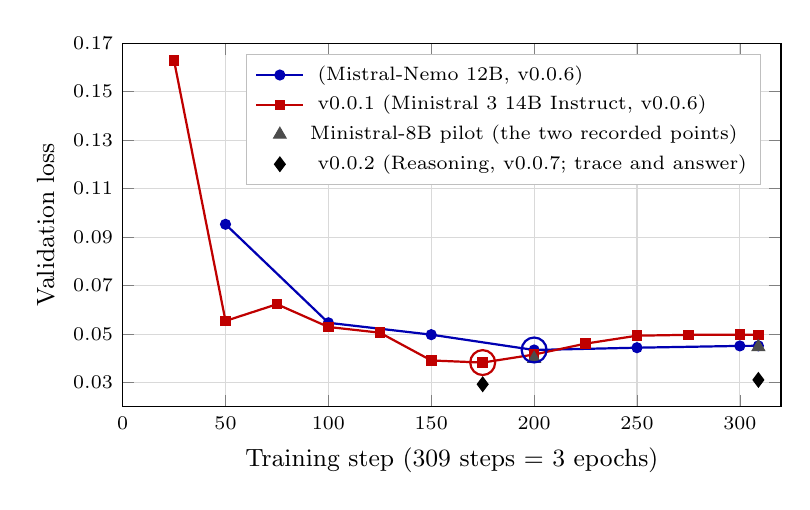
\begin{tikzpicture}
\begin{axis}[
  width=0.82\linewidth, height=6.2cm,
  xlabel={Training step (309 steps $=$ 3 epochs)}, ylabel={Validation loss},
  xmin=0, xmax=320, ymin=0.02, ymax=0.17,
  scaled y ticks=false, yticklabel style={/pgf/number format/fixed, /pgf/number format/precision=2},
  ytick={0.03,0.05,0.07,0.09,0.11,0.13,0.15,0.17},
  grid=major, grid style={gray!30},
  legend pos=north east, legend cell align=left,
  legend style={font=\scriptsize, draw=gray!50},
  tick label style={font=\scriptsize}, label style={font=\small},
]
\addplot[color=blue!70!black, mark=*, mark size=1.6pt, thick] coordinates {
  (50,0.09527) (100,0.05465) (150,0.04975) (200,0.04343) (250,0.04437) (300,0.04511) (309,0.04515)};
\addlegendentry{\hermes{} (Mistral-Nemo 12B, v0.0.6)}
\addplot[color=red!75!black, mark=square*, mark size=1.5pt, thick] coordinates {
  (25,0.16277) (50,0.05541) (75,0.06231) (100,0.05292) (125,0.05057) (150,0.03911) (175,0.03824)
  (200,0.04156) (225,0.04605) (250,0.04933) (275,0.04968) (300,0.04973) (309,0.04969)};
\addlegendentry{\logos{} v0.0.1 (Ministral 3 14B Instruct, v0.0.6)}
\addplot[color=gray!60!black, mark=triangle*, only marks, mark size=2.6pt] coordinates {(200,0.03987) (309,0.04469)};
\addlegendentry{Ministral-8B pilot (the two recorded points)}
\addplot[color=black, mark=diamond*, only marks, mark size=2.6pt] coordinates {(175,0.0293) (309,0.0311)};
\addlegendentry{\logos{} v0.0.2 (Reasoning, v0.0.7; trace and answer)}
\addplot[forget plot, color=blue!70!black, mark=o, only marks, mark size=4.5pt, thick] coordinates {(200,0.04343)};
\addplot[forget plot, color=red!75!black, mark=o, only marks, mark size=4.5pt, thick] coordinates {(175,0.03824)};
\end{axis}
\end{tikzpicture}
\caption{Validation loss by training step. Circles mark the checkpoints that were selected on validation loss and shipped: step 200 (epoch 1.95) for Hermes, 0.04343, and step 175 (epoch 1.70) for Logos v0.0.1, 0.03824. Both recorded curves rise through the third epoch, and in the other two runs the final value exceeds the selected one. The pilot and Logos v0.0.2 records keep only the best and final values; v0.0.2's loss covers the reasoning trace as well as the answer. The tokenizers differ between models, so the curves compare in shape, not in level.}
\label{fig:validation}
\end{figure}


\subsection{Checkpoint selection and resume verification}
% source: curves HER:137-154, L1:172-196, EXP:873-874, L2:88, 119-125; loss ratios HER:148-149, L1:193; fp16 skips HER:116, L1:147; gradient check HER:156-161, L1:200; adapters HER:193-196, L1:233-239, EXP:916-917; selection on the trace EXP:710-715; manifests AUD:61-70, HER:57-65.
Figure~\ref{fig:validation} shows the validation curves. In the two runs with a recorded curve, Hermes and Logos v0.0.1, the validation loss reaches its minimum before the end of the second epoch and rises through the third; the pilot and Logos v0.0.2 record only their best and final values, and in both the final value is above the selected one. The pilot and Hermes select step 200 (epoch 1.95), Logos v0.0.1 and v0.0.2 select step 175 (epoch 1.70). The final training loss sits about 10 times below the validation loss for Hermes and about 15 times below it for Logos v0.0.1, which is consistent with a third epoch that memorizes the 820 training targets; selection on validation loss keeps that epoch out of the shipped adapter. Two consequences were declared in advance. Logos' 25-step validation grid could select step 175 where Hermes' 50-step grid could not, and for Logos v0.0.2 the selection criterion covers the trace, which is 58\% of the validation targets by characters, so no answer-only validation loss exists for it. The optimizer skipped 4 steps on fp16 overflow during the Hermes run (through step 305) and 2 during Logos v0.0.1 (both before step 250); the pilot and v0.0.2 records do not report the count.

The interrupted runs were verified rather than assumed faithful. For Hermes, the gradient-check loss before training was bit-identical in both sessions (2.1058197021484375), the scheduler state carried over, and the two independent evaluations of step 300, one per session, agree to $1.4 \times 10^{-5}$ (0.045107 against 0.045121). For Logos v0.0.1, the first resume point was checked by size (368\,MB, a complete checkpoint) and the second file by file (weights, optimizer, scheduler, random-number and scaler state), and the final validation pass on the loaded best weights reproduced the recorded loss exactly. For Hermes and Logos v0.0.1 the exported adapter is byte-identical to the selected checkpoint's weights (SHA-256 \code{dc121fa3\ldots} and \code{f3e8dcdc\ldots}); for the pilot and Logos v0.0.2 the selected checkpoint is established from the recorded validation loss and the retained checkpoints, and v0.0.2's shipped adapter is \code{e49724f6\ldots} (Appendix~\ref{app:artifacts}). Each run's manifest records the hash of its full configuration, the git commit it ran at, the hash of the loaded dataset files and whether any configuration value was adjusted at runtime (none was).
